\chapter{Data generation}
To make the deception component generator a real one, it's necessary to have some data to insert into it.
For generate this datas i've used one of the most popular technology of our time: Large Language Models. In fact this is a task that they do well.
\\
As first step i've had to decide which LLM use: the model choosen is LLAMA2, principally because it's an open source project and it is possible to run it locally.
Done that i've used langchain \cite{langchain} to write a simple python script that generates the data. But before that it was necessary to find a way for use a LLM locally.
\section{Problem}
The benefit of running it locally have a cost: the precision of the model depends on the machine in which it's running. Eveni if the model is pretrained, depending on some parameters, the model could run better or worse.
\\\\
To fix this problem i had to choose in which way run the model. So two were the possible approaches:
\begin{itemize}
    \item use llama-cpp-python package
    \item use ollama
\end{itemize}
\begin{figure}[h]
    \caption{Llama-cpp data sample}
    \centering
    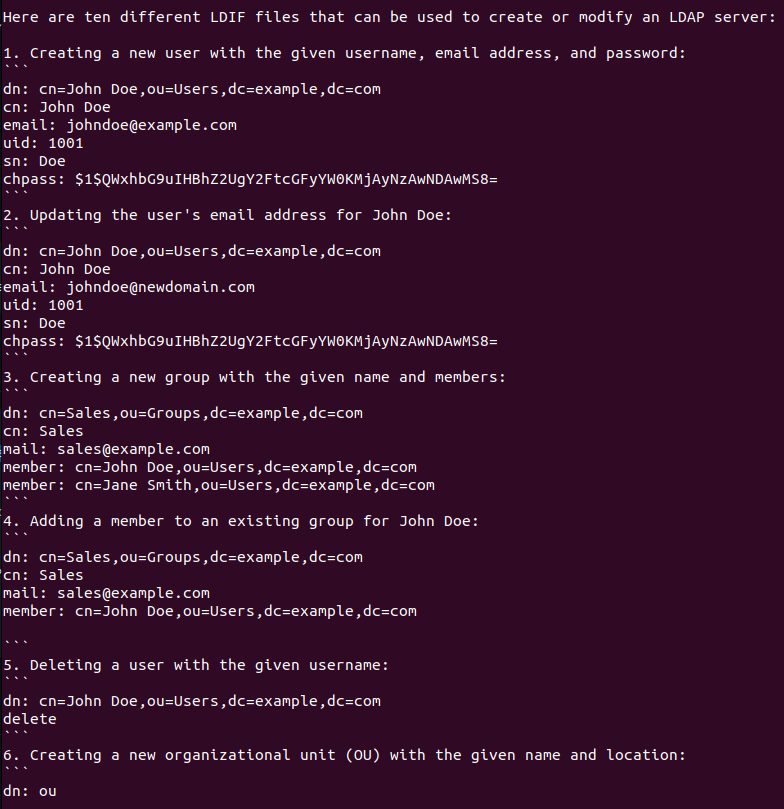
\includegraphics[width=8cm]{img/llamacpp.png}
\end{figure}
\section{llama-cpp-python}
This is a project born to create an interface to use llama-cpp in python \cite{llama-cpp-python}.
After setting up the environment, and create a python script to generate data (even inside the docker itself), what we can see is that the data generated are not so heterogeneous and it needs a lot of time to generate them.
Another negative aspect is that i've to download the model and insert it in the docker to make it run, so the docker grows in its weight.
\section{ollama}
To avoid all this problems i have decided to use Ollama \cite{ollama}. Ollama is a recent created project thatmakes users run LLMs locally in a docker-like way. So even in this case you have to download your model, but now we do not need to insert in our docker file.
\\
The idea is to generate data before, save it and then upload them in the docker.
Here we can see a more heterogeneous data creation. Even if there are changes to be made to make it works, it's bettere than the previous output.
\begin{figure}[h]
    \caption{Ollama data sample}
    \centering
    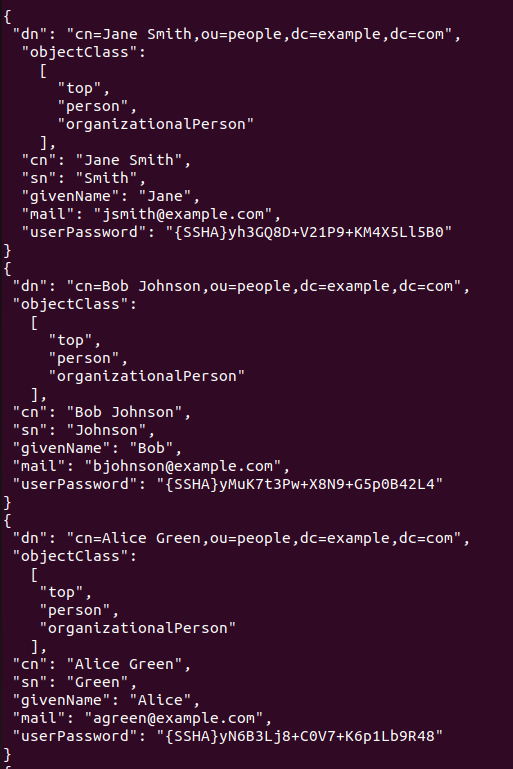
\includegraphics[width=8cm]{img/oll.png}
\end{figure}\\\\
After finding ollama, i've started to think on how i could implement it in a python script to make it generate random data when the docker is started.
\\
After reading the documentation online i've found a way to do so:
\begin{mdframed}[backgroundcolor=bpy]
\lstinputlisting[style=python]{code/ollama.py}
\end{mdframed}
\\\\
Analyzing that i've observed that it needs some time to run, but at least it creates a valid number of random data and in a more structured way (as we can see in the pictures reported). In that way it's easier to do some data cleaning to obtain a high quality output. 
\\
So now i've created the docker for the service, with the possibility to configure it and generate deception data: the last think to do is try to deploy it.
